\documentclass[12pt]{article}

\usepackage{amssymb,amsmath,amsthm}
\usepackage{bm}
\usepackage{graphicx,subcaption}
\usepackage[letterpaper, top=1in, left=1in, right=1in, bottom=1in]{geometry}

\newtheorem{definition}{Definition}
\newtheorem{theorem}{Theorem}
\newtheorem{lemma}{Lemma}
\newtheorem{remark}{Remark}

\title{\vspace{-4ex}\textbf{Construction of new distributions on embedded manifolds with an example on $\text{SO}(3)\times\mathbb{R}^n$}\vspace{-4ex}}
\date{}

\graphicspath{{./figs/}}

\begin{document}

\maketitle

\section{General idea} \label{sec:generalIdea}
The Von Mises distribution on unit circle $\mathbb{S}^1$, Von Mises-Fisher distribution on unit sphere $\mathbb{S}^n$, and Matrix Fisher distribution on Stiefel manifold $V_p(\mathbb{R}^n)$ can all be constructed from conditioning multivariate Gaussian distribution in their ambient Euclidean space onto the respective embedded manifolds.
The idea to construct distributions on the Cartesian product of these manifolds with extra Euclidean dimensions, i.e. $\mathbb{R}^{N_1}\times\mathcal{M}$, is similar.

Suppose $[\bm{x}_1^T,\bm{x}_2^T]^T$, follows multivariate Gaussian distributions with mean $[\bm{\mu}_1^T,\bm{\mu}_2^T]^T$, and covariance matrix $\mathbf{\Sigma} = \left[\begin{matrix}\mathbf{\Sigma}_1&\mathbf{P} \\\mathbf{P}^T&\mathbf{\Sigma}_2\end{matrix}\right]$, where $\bm{x}_1\in\mathbb{R}^{N_1}$ corresponds to the extra Euclidean dimensions, and $\bm{x}_2\in\mathbb{R}^{N_2}$ corresponds to the ambient Euclidean space of the manifold.
Then the density function can be calculated directly as:
\begin{equation} \label{eqn:MultiGaussian}
	\begin{split}
		f(\bm{x}_1,\bm{x}_2) = \frac{1}{\sqrt{(2\pi)^{N_1+N_2}|\mathbf{\Sigma}|}} &\text{exp}\left\{-\frac{1}{2}(\bm{x}_1-\bm{\mu}_c)^T\mathbf{\Sigma}_c^{-1}(\bm{x}_1-\bm{\mu}_c)\right\}\times \\
		&\text{exp}\left\{-\frac{1}{2}(\bm{x}_2-\bm{\mu}_2)^T\mathbf{\Sigma}_2^{-1}(\bm{x}_2-\bm{\mu}_2)\right\},
	\end{split}
\end{equation}
where $\bm{\mu}_c = \bm{\mu}_1+\mathbf{P}\mathbf{\Sigma}_2^{-1}(\bm{x}_2-\bm{\mu}_2)$, and $\mathbf{\Sigma}_c = \mathbf{\Sigma}_1-\mathbf{P}\mathbf{\Sigma}_2^{-1}\mathbf{P}^T$.
Let $g(\bm{x}_2)=\bm{0}$ be the constraint of the embedded manifold, the distribution on $\mathbb{R}^{n_1}\times\mathcal{M}$ is constructed by conditioning $(\bm{x}_1,\bm{x}_2)$ on $g(\bm{x}_2)=\bm{0}$.

Let $\mathcal{M}$ be an $m$-dimensional manifold, where $m<N_2$.
Then $g$ must have $N_2-m$ constraints.
However, the correlation terms between one extra Euclidean dimension and $\mathcal{M}$ given in $\mathbf{P}$ are of number $N_2$, which is larger than the dimensions of $\mathcal{M}$.
To mimic multivariate Gaussian distribution where correlations are linear and correspond to the dimensions of the Euclidean space, the correlation terms in \eqref{eqn:MultiGaussian} should be reduced to $m$ for one extra Euclidean dimension.
There is a geometric intuitive method to reduce the correlation terms: $\bm{x}_1$ and $\bm{x}_2$ should be only correlated in the tangent directions at the mean point $\bm{\mu}_2\in\mathcal{M}$.
The consequences of the correlation term in the tangent direction and orthogonal direction are shown in Figure \ref{fig:cylinder}.
It can be seen that the tangent correlation has the effect similar to the linear correlation in multivariate Gaussian distribution, whereas the orthogonal correlation behaves mostly in a non-linear fashion.

In a formal formulation, let $T_{\bm{\mu}_2}\mathcal{M}$ be the tangent space of $\mathcal{M}$ at $\bm{\mu}_2$.
Let $\bm{t}_1,\ldots,\bm{t}_m$ be an orthonormal basis of $T_{\bm{\mu}_2}\mathcal{M}$, and $\bm{n}_{m+1},\ldots,\bm{n}_{N_2}$ be its orthonormal complement in $\mathbb{R}^{N_2}$.
Let $\bm{e}_1,\ldots,\bm{e}_{N_2}$ be a natural orthonormal basis of $\mathbb{R}^{N_2}$, then there is a matrix $\mathbf{R}_t\in\mathrm{SO}(N_2)$ such that 
\begin{equation} \label{eqn:changeOfBasis}
\left[\begin{matrix}\bm{t}_1 & \cdots & \bm{t}_m & \bm{n}_{m+1} & \cdots & \bm{n}_{N_2} \end{matrix}\right]^T = \mathbf{R}_t \left[\begin{matrix}\bm{e}_1 & \cdots & \bm{e}_{N_2}\end{matrix}\right]^T
\end{equation}
if they are placed in some proper right-hand order.
Let $x_{1i}$ be a component of $\bm{x}_1$, $x_{2j}$ be a component of $\bm{x}_2$ in the $\{\bm{e}_1,\ldots,\bm{e}_{N_2}\}$ coordinate system, and $\tilde{x}_{2j}$ be a component of $\bm{x}_2$ in the $\{\bm{t}_1,\ldots,\bm{t}_m,\bm{n}_{m+1},\ldots,\bm{n}_{N_2}\}$ coordinate system.
Then $[\begin{matrix}x_{21} & \ldots & x_{2N_2}\end{matrix}] = [\begin{matrix}\tilde{x}_{21} & \ldots & \tilde{x}_{2N_2}\end{matrix}]\mathbf{R}_t$.
Because of the bi-linearity of covariance, this leads to
\begin{equation}
	\left[\begin{matrix}
	\text{cov}(x_{1i},x_{21}) & \ldots & \text{cov}(x_{1i},x_{2N_2})
	\end{matrix}\right] = \left[\begin{matrix}
	\text{cov}(x_{1i},\tilde{x}_{21}) & \ldots & \text{cov}(x_{1i},\tilde{x}_{2N_2})
	\end{matrix}\right]\mathbf{R}_t,
\end{equation}
where the left-hand side is the $i$-th row of covariance matrix $\mathbf{P}$.
By the intuition from last paragraph, let $\mathrm{cov}(x_{1i},\tilde{x}_{21})=\tilde{P}_{i1}, \; \ldots, \; \mathrm{cov}(x_{1i},\tilde{x}_{2m})=\tilde{P}_{im}$ be the $m$ correlation terms between $x_{1i}$ and $\bm{x}_2$ conditioned on $g(\bm{x}_2)=\bm{0}$, and $\mathrm{cov}(x_{1i},\tilde{x}_{2j}) = 0$ for $j=m+1,\ldots,N_2$.
Then the $i$-th row of the covariance matrix $\mathbf{P}$ and the reduced correlation terms have relationship:
\begin{equation} \label{eqn:reduceCorrelation}
	\left[\begin{matrix}
	\text{cov}(x_{1i},x_{21}) & \ldots & \text{cov}(x_{1i},x_{2N_2})
	\end{matrix}\right] = \left[\begin{matrix}
	\tilde{P}_{i1} & \ldots & \tilde{P}_{im} & 0 & \ldots & 0)
	\end{matrix}\right]\mathbf{R}_t,
\end{equation}
which is the equation for reducing the correlation terms.

\begin{figure*}[t!]
	\centering
	\begin{subfigure}[t]{0.5\textwidth}
		\centering
		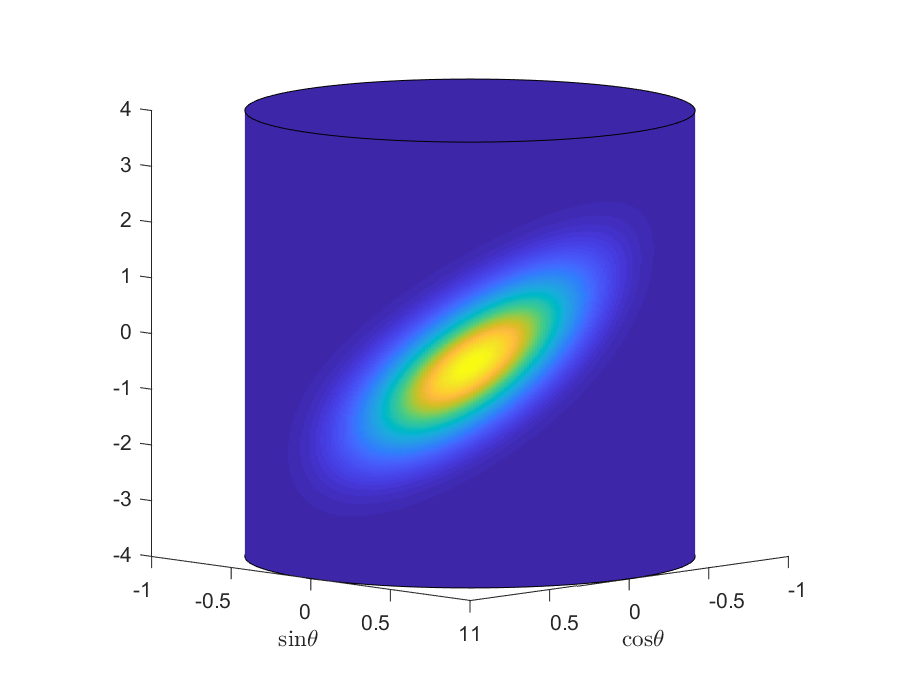
\includegraphics[height=2in]{cylinder-tangent}
		\caption{Correlation in tangent direction}
	\end{subfigure}%
	\hfill
	\begin{subfigure}[t]{0.5\textwidth}
		\centering
		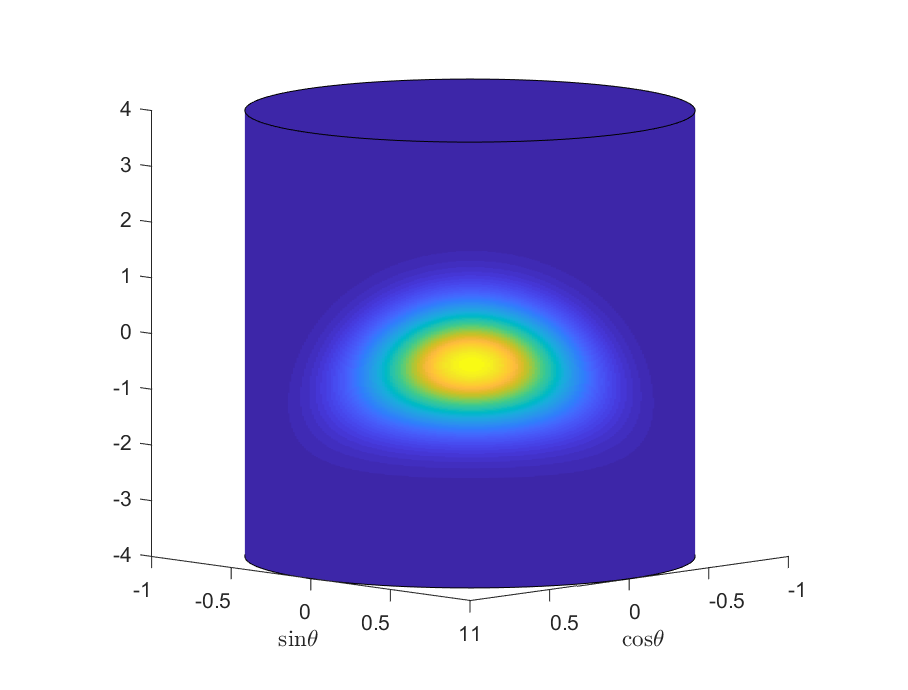
\includegraphics[height=2in]{cylinder-normal}
		\caption{Correlation in normal direction}
	\end{subfigure}
	\caption{Conditioning tri-variate Gaussian distribution on cylinder. \label{fig:cylinder}}
\end{figure*}


\section{Matrix Fisher Distribution on SO(3) \label{sec:MatrixFisher}}
Before constructing a distribution on SO(3)$\times\mathbb{R}^n$, let us first look at how the Matrix Fisher distribution on SO(3) is constructed by conditioning multivariate Gaussian distribution.
To construct Matrix Fisher distribution on SO(3), we need a nine dimensional Euclidean space, i.e. $\bm{x}_2\in\mathbb{R}^{9}$.

There are two constraint functions of SO(3), $g_1(\bm{x}_2) = \mathrm{vec}^{-1}(\bm{x}_2)^T\mathrm{vec}^{-1}(\bm{x}_2)-\mathbf{I}_{3\times 3}$ and $g_2(\bm{x}_2) = \mathrm{det}(\mathrm{vec}^{-1}(\bm{x}_2))-1$.
Let $\mathrm{vec}^{-1}(\bm{\mu}_2)^T = \mathbf{M}^\prime\in\mathrm{O}(3)$, and
\begin{equation} \label{eqn:sigma2}
\mathbf{\Sigma}_2 = \left[\begin{matrix}
\mathbf{K}^{\prime-1} & \mathbf{0} & \mathbf{0} \\
\mathbf{0} & \mathbf{K}^{\prime-1} & \mathbf{0} \\
\mathbf{0} & \mathbf{0} & \mathbf{K}^{\prime-1}
\end{matrix}\right]
\end{equation}
where $\mathbf{K}^\prime\in\mathbb{R}^{3\times3}$ is symmetric positive semi-definite but not necessarily diagonal.
By conditioning $(\bm{x}_1,\bm{x}_2)$ on $g_1(\bm{x}_2)=\bm{0}$ and $g_2(\bm{x}_2)=0$, the second exponential term in \eqref{eqn:MultiGaussian} becomes
\begin{equation}
\begin{split}
-\frac{1}{2}(\bm{x}_2-\bm{\mu}_2)^T\mathbf{\Sigma}_2^{-1}(\bm{x}_2-\bm{\mu}_2) &= \mathrm{tr}\left(-\frac{1}{2}\mathbf{K}^\prime(\mathrm{vec}^{-1}(\bm{x}_2)^T-\mathbf{M}^\prime)^T(\mathrm{vec}^{-1}(\bm{x}_2)^T-\mathbf{M}^\prime)\right) \\
&\propto \mathrm{tr}(\mathbf{M}^\prime\mathbf{K}^\prime\mathrm{vec}^{-1}(\bm{x}_2)),
\end{split}
\end{equation}
where $\mathbf{M}^\prime\mathbf{K}^\prime=\mathbf{F}$ is the parameter for the Matrix Fisher distribution, and $\mathrm{vec}^{-1}(\bm{x}_2)=\mathbf{R}^T$ is a rotation matrix.
It should be noted the mean value $\mathbf{M}^\prime$ is in O(3), not limited to SO(3), this makes the distribution far richer, including some degenerated cases which cannot be represented if $\mathbf{M}^\prime\in\mathrm{SO}(3)$.
The above definition is equivalent to the usual definition of Matrix Fisher distribution because every $\mathbf{F}\in\mathbb{R}^{3\times 3}$ has a polar decomposition as $\mathbf{M}^\prime\mathbf{K}^\prime$.
Also note that when $\mathbf{K}^\prime$ is only positive semi-definite, $\mathbf{K}^{\prime-1}$ is not defined, but the Matrix Fisher distribution is still well-defined, this corresponds to the limiting case of ``uniform distribution in Euclidean space".

The singular value decomposition of $\mathbf{F} = \mathbf{U^\prime}\mathbf{S^\prime}\mathbf{V}^T$ can be defined in different ways.
First, assume $\mathbf{S}^\prime = \mathrm{diag}(s_1,\ s_2,\ s_3)$ has non-negative diagonal entries.
Since the decomposition is invariant under simultaneous sign change of the corresponding columns of $\mathbf{U}^\prime$ and $\mathbf{V}$, we impose uniqueness condition on $\mathbf{V}$ such that the first non-zero element of each column of $\mathbf{V}$ is positive; and then if $\mathrm{det}(\mathbf{V})=-1$, we flip the sign of the third column.
With this convention, the SVD of $\mathbf{F}$ is unique if $s_1$, $s_2$, $s_3$ are different, and $\mathbf{K}^\prime = \mathbf{V}\mathbf{S}^\prime\mathbf{V}^T$ is positive semi-definite, $\mathbf{M}^\prime = \mathbf{U}^\prime\mathbf{V}^T\in\mathrm{O}(3)$.
Second, if $\mathrm{det}(\mathbf{U}^\prime)=-1$, let $\mathbf{U} = \mathbf{U}^\prime\mathrm{diag}(1,1,-1)$, and $\mathbf{S} = \mathbf{S}^\prime\mathrm{diag}(1,1,-1)$.
Then $\mathbf{F} = \mathbf{U}\mathbf{S}\mathbf{V}^T$ is the unique proper singular value decomposition if $\mathbf{F}$ does not have repeated eigenvalues.


\section{An example on SO(3)$\times\mathbb{R}^N$}

Let $\frac{1}{\sqrt{2}}\hat{\bm{e}}_1$, $\frac{1}{\sqrt{2}}\hat{\bm{e}}_2$ and $\frac{1}{\sqrt{2}}\hat{\bm{e}}_3$ be the natural orthonormal basis of $\mathfrak{so}$(3).
Then a orthonormal basis of the tangent space at the mean attitude $\mathbf{M}$ is $\frac{1}{\sqrt{2}}\mathbf{M}\widehat{\mathbf{V}\bm{e}_1}$, $\frac{1}{\sqrt{2}}\mathbf{M}\widehat{\mathbf{V}\bm{e}_2}$, $\frac{1}{\sqrt{2}}\mathbf{M}\widehat{\mathbf{V}\bm{e}_3}$.
With the intuition from Section \ref{sec:generalIdea}, the distribution (Matrix Fisher-Gaussian) on SO(3)$\times\mathbb{R}^N$ can be defined as follows:

\begin{definition}
	$(\bm{x},\mathbf{R})\in\mathbb{R}^N\times\mathrm{SO}(3)$ follows Matrix Fisher-Gaussian distribution with parameters $\bm{\mu}\in\mathbb{R}^N$, $\mathbf{\Sigma}\in\mathbb{R}^{N\times N}$, $\mathbf{U},\mathbf{V}\in\mathrm{SO}(3)$, $\mathbf{S}\in\mathbb{R}^{3\times 3}$ and $\tilde{\mathbf{P}}\in\mathbb{R}^{N\times 3}$ if and only if it has density function:
	\begin{equation} \label{eqn:MFG}
		f(\bm{x},\mathbf{R};\bm{\mu},\mathbf{\Sigma},\mathbf{V},\mathbf{S},\mathbf{U},\tilde{\mathbf{P}}) = \frac{1}{c(\mathbf{F})\sqrt{(2\pi)^n|\mathbf{\Sigma}_c|}} \mathrm{exp}\left\{-\frac{1}{2}(\bm{x}-\bm{\mu}_c)^T\mathbf{\Sigma}_c^{-1}(\bm{x}-\bm{\mu}_c)\right\} \mathrm{etr}\left\{\mathbf{F}\mathbf{R}^T\right\},
	\end{equation}
	where $\mathbf{F} = \mathbf{U}\mathbf{S}\mathbf{V}^T$, $\bm{\mu}_c = \bm{\mu}+\mathbf{P}\mathbf{\Sigma}_2^{-1}(\mathrm{vec}(\mathbf{R}^T)-\bm{\mu}_2)$, and $\mathbf{\Sigma}_c = \mathbf{\Sigma}-\mathbf{P}\mathbf{\Sigma}_2^{-1}\mathbf{P}^T$ with $\bm{\mu}_2=\mathrm{vec}(\mathbf{V}\mathbf{U}^T)$ and $\mathbf{\Sigma}_2$ is given in \eqref{eqn:sigma2} in which $\mathbf{K} = \mathbf{V}\mathbf{S}\mathbf{V}^T$.
	Let $\bm{t}_{1:3}=\frac{1}{\sqrt{2}} \mathrm{vec}[(\mathbf{U}\mathbf{V}^T\widehat{\mathbf{V}\bm{e}_{1:3}})^T]$, $\bm{n}_{4:9}$ be its orthonormal complement in $\mathbb{R}^9$, $\mathbf{R}_t$ given in \eqref{eqn:changeOfBasis}, then the $i$-th row of $\mathbf{P}$ is given in \eqref{eqn:reduceCorrelation} with $[\begin{matrix}\tilde{P}_{i1} & \tilde{P}_{i2} & \tilde{P}_{i3}\end{matrix}]$ given by the $i$-th row of $\tilde{\mathbf{P}}$.
\end{definition}

The above definition seems complicated, but it is simple in the way that the marginal distribution of $\mathbf{R}$ is Matrix-Fisher distribution, and the conditional distribution of $\bm{x}$ is Gaussian distribution.
And the correlation parameter $\tilde{\mathbf{P}}$ is defined to mimic the linear correlation in Euclidean space.
This can be seen from Figure \ref{fig:SO3Correlation} with $N=1$, $\mu=0$, $\Sigma=1$, $\mathbf{F}=10\mathbf{I}_{3\times 3}$.
If the correlation is only in $\bm{t}_1$ direction, when $x$ becomes larger, the distribution rotates about $\bm{e}_1$-axis a little bit; when $x$ becomes smaller, the distribution rotates about $\bm{e}_1$-axis in the reverse direction a little bit.
This is also the case for the correlation in $\bm{t}_2$ and $\bm{t}_3$ directions.
However, the conditional distribution of $\mathbf{R}$ shown in Figure \ref{fig:SO3Correlation} is no longer Matrix Fisher distribution, it involves the second order terms of $\mathbf{R}$ as indicated in \eqref{eqn:MFG}.

To make Matrix-Fisher Gaussian distribution well defined, the parameters should satisfy certain conditions as stated in the next theorem.
\begin{theorem} \label{thm:PTildeRange}
	The Matrix Fisher-Gaussian distribution is well defined if $\mathbf{\Sigma}\succ 0$, $\mathbf{S}=\mathrm{diag}(s_1,\ s_2,\ s_3)$ where $s_1>s_2>|s_3|>0$, and $\mathbf{\Sigma}-\frac{1}{2}\tilde{\mathbf{P}}\mathrm{diag}(s_2+s_3,\ s_1+s_3,\ s_1+s_2)\tilde{\mathbf{P}}^T \succ 0$.
\end{theorem}
\begin{proof}
	From the knowledge of common Matrix Fisher distribution and Gaussian distribution, Matrix Fisher-Gaussian distribution is well defined if $\mathbf{\Sigma}$, $\mathbf{S}$ satisfy the conditions stated in the theorem, and $\mathbf{\Sigma}_c\succ 0$.
	Substitute \eqref{eqn:reduceCorrelation} into the expression for $\mathbf{\Sigma}_c$, we get:
	\begin{equation}
		\mathbf{\Sigma}_c = \mathbf{\Sigma}_1 - \tilde{\mathbf{P}}\begin{bmatrix}
			\bm{t}^T_1 \\ \bm{t}^T_2 \\ \bm{t}^T_3
		\end{bmatrix}\begin{bmatrix}
			\mathbf{K} & \mathbf{0} & \mathbf{0} \\
			\mathbf{0} & \mathbf{K} & \mathbf{0} \\
			\mathbf{0} & \mathbf{0} & \mathbf{K}
		\end{bmatrix}\begin{bmatrix}
			\bm{t}_1 & \bm{t}_2 & \bm{t}_3
		\end{bmatrix}\tilde{\mathbf{P}}^T.
	\end{equation}
	Let $\tilde{\mathbf{\Sigma}}^{-1}_2$ be the term between $\tilde{\mathbf{P}}$ and $\tilde{\mathbf{P}}^T$, write $\bm{t}^T_i$ = $\begin{bmatrix}\bm{t}^T_{i1}&\bm{t}^T_{i2}&\bm{t}^T_{i3}\end{bmatrix}$ such that $\bm{t}_{ik}\in\mathbb{R}^3$, then the $i,j$-th entry of $\tilde{\mathbf{\Sigma}}^{-1}_2$ is given by:
	\begin{equation} \label{eqn:sigma2Entry}
		\begin{split}
			(\tilde{\mathbf{\Sigma}}^{-1}_2)_{ij} &= \sum_{k=1}^{3}\bm{t}^T_{ik}\mathbf{K}\bm{t}_{jk} = \mathrm{tr}\left(\begin{bmatrix}
				\bm{t}^T_{i1} \\ \bm{t}^T_{i2} \\ \bm{t}^T_{i3}
			\end{bmatrix}\mathbf{K}\begin{bmatrix}
				\bm{t}_{j1} & \bm{t}_{j2} & \bm{t}_{j3}
			\end{bmatrix}\right) \\
			&= \frac{1}{2}\mathrm{tr}(\mathbf{U}\mathbf{V}^T\widehat{\mathbf{V}\bm{e}_i}\mathbf{K}\widehat{\mathbf{V}\bm{e}_j}^T\mathbf{V}\mathbf{U}^T) = \frac{1}{2}\mathrm{tr}(\mathbf{S}\hat{\bm{e}}_j^T\hat{\bm{e}}_i) \\
		\end{split}
	\end{equation}
	This proves $\tilde{\mathbf{\Sigma}}^{-1}_2 = \frac{1}{2}\mathrm{diag}(s_2+s_3,\ s_1+s_3,\ s_1+s_2)$.
\end{proof}
The above theorem indicates the range of $\tilde{\mathbf{P}}$ is the same as the covariance matrix between an $N$-variate Gaussian distribution with covariance $\mathbf{\Sigma}$, and a tri-variate Gaussian distribution with covariance $\tilde{\mathbf{\Sigma}}_2$.
In fact, this argument is even stronger, as we will show in the next theorem that the Matrix Fisher-Gaussian distribution can be approximated by a six dimensional Gaussian distribution if the Matrix Fisher part is highly concentrated.
\begin{theorem}
	Let $\mathbf{R} = \mathbf{U}\mathbf{V}^T\mathrm{exp}(\widehat{\mathbf{V}\bm{\eta}})$, if $(\bm{x},\mathbf{R})$ follows Matrix Fisher-Gaussian distribution with $|s_3|\gg 0$, then $(\bm{x},\bm{\eta})$ approximately follows a six dimensional Gaussian distribution with mean $\left(\bm{\mu},\mathbf{0}\right)$ and covariance matrix $\begin{bmatrix}
		\mathbf{\Sigma} & \frac{1}{\sqrt{2}}\tilde{\mathbf{P}} \\
		\frac{1}{\sqrt{2}}\tilde{\mathbf{P}}^T & \frac{1}{2}\tilde{\mathbf{\Sigma}}_2
	\end{bmatrix}$.
\end{theorem}
\begin{proof}
	It has been shown if $|s_3|\gg 0$, the Matrix Fisher part can be approximated by $\bm{\eta}\sim \mathcal{N}(\mathbf{0},\frac{1}{2}\tilde{\mathbf{\Sigma}})$.
	From \eqref{eqn:MFG}, $\bm{x}|\bm{\eta}\sim \mathcal{N}(\bm{\mu}_c,\mathbf{\Sigma}_c)$, and it has been shown in the last theorem $\mathbf{\Sigma}_c = \mathbf{\Sigma}-\tilde{\mathbf{P}}\tilde{\mathbf{\Sigma}}_2^{-1}\tilde{\mathbf{P}}^T$.
	Furthermore, $\bm{\mu}_c$ has the following approximation
	\begin{equation}
		\label{eqn:linearApprox}
		\begin{split}
			\bm{\mu}_c &= \bm{\mu} + \tilde{\mathbf{P}}\begin{bmatrix}
				\bm{t}_1 & \bm{t}_2 & \bm{t}_3
			\end{bmatrix}^T\mathbf{\Sigma}_2^{-1} \mathrm{vec}\left(\mathrm{exp}(\widehat{\mathbf{V}\bm{\eta}})^T\mathbf{V}\mathbf{U}^T-\mathbf{V}\mathbf{U}^T\right) \\
			&\approx \bm{\mu} + \tilde{\mathbf{P}}\begin{bmatrix}
				\bm{t}_1 & \bm{t}_2 & \bm{t}_3
			\end{bmatrix}^T\mathbf{\Sigma}_2^{-1} \mathrm{vec}\left((\mathbf{I}_{3\times 3}+\widehat{\mathbf{V}\bm{\eta}}^T)\mathbf{V}\mathbf{U}^T-\mathbf{V}\mathbf{U}^T\right)\\
			&= \bm{\mu} + \tilde{\mathbf{P}}\begin{bmatrix}
				\bm{t}_1 & \bm{t}_2 & \bm{t}_3
			\end{bmatrix}^T\mathbf{\Sigma}_2^{-1}\begin{bmatrix}
				\bm{t}_1 & \bm{t}_2 & \bm{t}_3
			\end{bmatrix}(\sqrt{2}\bm{\eta}) \\
			&= \bm{\mu} + \sqrt{2}\tilde{\mathbf{P}}\tilde{\mathbf{\Sigma}}_2^{-1}\bm{\eta}
		\end{split},
	\end{equation}
	where the third equation uses the fact that the tangent space is a vector space.
	This finishes the proof since $\bm{x}|\bm{\eta}$ is approximated by the conditional distribution of the desired six dimensional Gaussian distribution.
\end{proof}

The Matrix Fisher-Gaussian distribution is defined on a nonlinear manifold, so its intact form cannot be represented by a six dimensional Gaussian distribution, although it has six degrees of freedom.
However, combining Theorem \ref{thm:PTildeRange} and the next theorem, we can show it in some way resembles a six dimensional Gaussian distribution.
\begin{theorem} \label{thm:Miuc}
	$\bm{\mu}_c = \bm{\mu} + \frac{1}{\sqrt{2}}\tilde{\mathbf{P}}\begin{bmatrix}
		\mathrm{tr}\left(\mathbf{S}\mathrm{exp}(\hat{\bm{\eta}})^T\hat{\bm{e}}_1\right) \\
		\mathrm{tr}\left(\mathbf{S}\mathrm{exp}(\hat{\bm{\eta}})^T\hat{\bm{e}}_2\right) \\
		\mathrm{tr}\left(\mathbf{S}\mathrm{exp}(\hat{\bm{\eta}})^T\hat{\bm{e}}_3\right)
	\end{bmatrix}^T \triangleq \bm{\mu}+\tilde{\mathbf{P}}f(\bm{\eta})$.
\end{theorem}
\begin{proof}
	\begin{equation}
		\bm{\mu}_c = \bm{\mu} + \tilde{\mathbf{P}}\begin{bmatrix}
		\bm{t}_1 & \bm{t}_2 & \bm{t}_3
		\end{bmatrix}^T\mathbf{\Sigma}_2^{-1} \mathrm{vec}\left(\mathrm{exp}(\widehat{\mathbf{V}\bm{\eta}})^T\mathbf{V}\mathbf{U}^T-\mathbf{V}\mathbf{U}^T\right),
	\end{equation}
	and 
	\begin{equation}
		\begin{split}
			&\bm{t}_i^T\mathbf{\Sigma}_2^{-1}\mathrm{vec}\left(\mathrm{exp}(\widehat{\mathbf{V}\bm{\eta}})^T\mathbf{V}\mathbf{U}^T-\mathbf{V}\mathbf{U}^T\right) \\
			= &\frac{1}{\sqrt{2}}\mathrm{tr}\left\{\mathbf{U}\mathbf{V}^T\widehat{\mathbf{V}\bm{e}_i}\mathbf{K}\left(\mathrm{exp}(\widehat{\mathbf{V}\bm{\eta}})^T\mathbf{V}\mathbf{U}^T-\mathbf{V}\mathbf{U}^T\right)\right\} \\
			= &\frac{1}{\sqrt{2}}\mathrm{tr}\left\{\mathbf{V}\hat{\bm{e}}_i\mathbf{V}^T\mathbf{V}\mathbf{S}\mathbf{V}^T\left(\mathbf{V}\mathrm{exp}(\hat{\bm{\eta}})^T\mathbf{V}^T+\mathbf{I}\right)\right\} \\
			= &\frac{1}{\sqrt{2}}\mathrm{tr}\left(\mathbf{S}\mathrm{exp}(\hat{\bm{\eta}})^T\hat{\bm{e}}_i + \mathbf{S}\hat{\bm{e}}_i\right),
		\end{split}
	\end{equation}
	where the second term vanishes.
\end{proof}

Compared to \eqref{eqn:linearApprox}, the nice linear term $\sqrt{2}\tilde{\mathbf{\Sigma}}_2^{-1}\bm{\eta}$ is replaced by the nonlinear term $f(\bm{\eta})$, which is the consequence of the non-linearity of SO(3).
Because of the non-uniqueness of singular value decomposition when $\mathbf{F}\mathbf{F}^T$ has repeated eigenvalues, the parameters of Matrix Fisher-Gaussian distribution is sometimes redundant.
For example, when $\mathbf{F} = s_1\mathbf{I}$, $\mathbf{V}$ can be arbitrary, and $\tilde{\mathbf{P}}$ can be defined with respect to different $\mathbf{V}$.
However, if $\tilde{\mathbf{P}}$ is chosen carefully such that $\mathbf{P}$ stays the same, the distribution is unchanged.
To deal with this non-uniqueness problem, we give the equivalent conditions of Matrix Fisher-Gaussian distribution in the following theorem.
\begin{theorem} \label{thm:Equivalence}
	Two Matrix Fisher-Gaussian distributions with parameters $(\bm{\mu}_\alpha, \mathbf{\Sigma}_\alpha, \mathbf{U}_\alpha, \mathbf{S}_\alpha, \mathbf{V}_\alpha, \mathbf{\tilde{P}}_\alpha)$ and $(\bm{\mu}_\beta, \mathbf{\Sigma}_\beta, \mathbf{U}_\beta, \mathbf{S}_\beta, \mathbf{V}_\beta, \mathbf{\tilde{P}}_\beta)$ are equivalent if and only if $\bm{\mu}_\alpha=\bm{\mu}_\beta$, $\mathbf{S}_\alpha=\mathbf{S}_\beta$ and if
	\begin{enumerate}
		\item $s_{\alpha 1}=s_{\alpha 2}=s_{\alpha 3}=0$, $\mathbf{\Sigma}_\alpha=\mathbf{\Sigma}_\beta$;
		\item $s_{\alpha 1}=s_{\alpha 2}=s_{\alpha 3}\neq 0$, $\exists\mathbf{T}\in\mathrm{SO}(3)$ such that $\mathbf{U}_\beta=\mathbf{U}_\alpha\mathbf{T}$, $\mathbf{V}_\beta=\mathbf{V}_\alpha\mathbf{T}$, $\tilde{\mathbf{P}}_\beta=\tilde{\mathbf{P}}_\alpha\mathbf{T}$ and $\mathbf{\Sigma}_\alpha=\mathbf{\Sigma}_\beta$;
		\item $s_{\alpha 1}=s_{\alpha 2}=-s_{\alpha 3}\neq 0$, $\exists\mathbf{T}\in\mathrm{O}(3)\setminus\mathrm{SO}(3)$ such that $\mathbf{U}_\beta=\mathbf{U}_\alpha\mathbf{T}\mathbf{D}_3$, $\mathbf{V}_\beta=\mathbf{V}_\alpha\mathbf{D}_3\mathbf{T}$, $\tilde{\mathbf{P}}_\beta=\tilde{\mathbf{P}}_\alpha\mathbf{T}\mathbf{D}_3$, and $\mathbf{\Sigma}_\beta=\mathbf{\Sigma}_\alpha+\tilde{\mathbf{P}}_\alpha\left(\mathbf{T}\tilde{\mathbf{\Sigma}}_{2\alpha}^{-1}\mathbf{T}^T-\tilde{\mathbf{\Sigma}}_{2\alpha}^{-1}\right)\tilde{\mathbf{P}}_\alpha^T$, where $\mathbf{D}_3=\begin{bmatrix}1&0&0\\0&1&0\\0&0&-1\end{bmatrix}$;
		\item $s_{\alpha 1}\neq s_{\alpha 2}=s_{\alpha 3}=0$, $\mathbf{U}_\beta=\mathbf{U}_\alpha\mathrm{exp}(\theta\hat{\bm{e}_1})$, $\mathbf{V}_\beta=\mathbf{V}_\alpha\mathrm{exp}(\theta\hat{\bm{e}_1})$ for some $\theta\in\mathbb{R}$, $[\tilde{\mathbf{P}}_{\beta, :2}, \tilde{\mathbf{P}}_{\beta, :3}] = [\tilde{\mathbf{P}}_{\alpha, :2}, \tilde{\mathbf{P}}_{\alpha, :3}]\begin{bmatrix}\cos\theta&\sin\theta\\-\sin\theta&\cos\theta\end{bmatrix}$, and $\mathbf{\Sigma}_\alpha=\mathbf{\Sigma}_\beta$, where $\tilde{P}_{:i}$ denotes its $i$-th column.
		\item $s_{\alpha 1}\neq s_{\alpha 2}=s_{\alpha 3}\neq 0$, $\mathbf{U}_\beta=\mathbf{U}_\alpha\mathrm{exp}(\theta\hat{\bm{e}_1})$, $\mathbf{V}_\beta=\mathbf{V}_\alpha\mathrm{exp}(\theta\hat{\bm{e}_1})$ for some $\theta\in\mathbb{R}$, $\tilde{\mathbf{P}}_\beta=\tilde{\mathbf{P}}_\alpha\mathrm{exp}(\theta\hat{\bm{e}_1})$, and $\mathbf{\Sigma}_\alpha=\mathbf{\Sigma}_\beta$;
		\item $s_{\alpha 1}\neq s_{\alpha 2}=-s_{\alpha 3}\neq 0$, $\mathbf{U}_\beta=\mathbf{U}_\alpha\mathrm{exp}(\theta\hat{\bm{e}_1})$, $\mathbf{V}_\beta=\mathbf{V}_\alpha\mathrm{exp}(\theta\hat{\bm{e}_1})^T$ for some $\theta\in\mathbb{R}$, $\tilde{\mathbf{P}}_\beta=\tilde{\mathbf{P}}_\alpha\mathrm{exp}(\theta\hat{\bm{e}_1})$, and $\mathbf{\Sigma}_\beta=\mathbf{\Sigma}_\alpha+\tilde{\mathbf{P}}_\alpha\left(\mathrm{exp}(\theta\hat{\bm{e}_1})\tilde{\mathbf{\Sigma}}_{2\alpha}^{-1}\mathrm{exp}(\theta\hat{\bm{e}_1})^T-\tilde{\mathbf{\Sigma}}_{2\alpha}^{-1}\right)\tilde{\mathbf{P}}_\alpha^T$;
		\item $s_{\alpha 1}=s_{\alpha 2}\neq|s_{\alpha 3}|$, $\mathbf{U}_\beta=\mathbf{U}_\alpha\mathrm{exp}(\theta\hat{\bm{e}_3})$, $\mathbf{V}_\beta=\mathbf{V}_\alpha\mathrm{exp}(\theta\hat{\bm{e}_3})^T$ for some $\theta\in\mathbb{R}$, $\tilde{\mathbf{P}}_\beta=\tilde{\mathbf{P}}_\alpha\mathrm{exp}(\theta\hat{\bm{e}_3})$ and $\mathbf{\Sigma}_\alpha=\mathbf{\Sigma}_\beta$;
		\item $s_{\alpha 1}\neq s_{\alpha 2}\neq |s_{\alpha 3}|$, $\mathbf{U}_\alpha=\mathbf{U}_\beta$, $\mathbf{V}_\alpha=\mathbf{V}_\beta$, $\tilde{\mathbf{P}}_\alpha=\tilde{\mathbf{P}}_\beta$, and $\mathbf{\Sigma}_\alpha=\mathbf{\Sigma}_\beta$.
	\end{enumerate}
\end{theorem}
The proof of this theorem is given in Appendix \ref{apd:proof}.
It can be seen that when $\mathbf{F}\mathbf{F}^T$ has repeated eigenvalues, the equivalent conditions of Matrix Fisher-Gaussian distribution become complicated.
And surprisingly, when $s_2=-s_3$, two distributions can be equivalent even if they have different covariance matrices for the Gaussian part.


\section{Maximum Likelihood Estimator}
Let $(\bm{x}_n,\mathbf{R}_n)_{n=1}^{N_s}$ be $N_s$ independent samples from Matrix Fisher-Gaussian distribution with weights $w_n$ such that $\sum_{n=1}^{N_s}w_n=1$.
Then the maximum likelihood estimator of the parameters of Matrix Fisher-Gaussian distribution is given by the following theorem.

\begin{theorem}
	\label{thm:MLE}
	Let $\mathrm{E}_s(\mathbf{R}) = \sum_{n=1}^{N_s}w_n\mathbf{R}_n$ be the sample mean of the rotation matrices, and $\mathbf{U}_s\mathbf{D}_s\mathbf{V}_s^T=\mathrm{E}_s(\mathbf{R})$ be its proper singular value decomposition (unique almost surely), then the maximum likelihood estimation for the Matrix Fisher part is:
	\begin{equation} \label{eqn:MLEMatrixFisher}
		\hat{\mathbf{U}} = \mathbf{U}_s, \qquad \hat{\mathbf{V}} = \mathbf{V}_s, \qquad d_i = \frac{1}{c(\hat{\mathbf{S}})}\frac{\partial c(\hat{\mathbf{S}})}{\partial \hat{s}_i},
	\end{equation}
	where $\mathrm{diag}(d_1,\ d_2,\ d_3) = \mathbf{D}_s$.
	Then define $\mathrm{exp}(\bm{\eta}_n) = \hat{\mathbf{U}}^T\mathbf{R}_n\hat{\mathbf{V}}$ for $n=1,\ldots,N_s$, and the following sample moments:
	\begin{align*}
		&\mathrm{E}_s(\bm{x}) = \sum_{n=1}^{N_s}w_n\bm{x}_n, \qquad \mathrm{cov}_s(\bm{x},\bm{x}) = \sum_{n=1}^{N_s}w_n\bm{x}_n\bm{x}_n^T-\mathrm{E}_s(\bm{x})\mathrm{E}_s(\bm{x})^T, \\
		&\mathrm{E}_s(f(\bm{\eta})) = \sum_{n=1}^{N_s}w_nf(\bm{\eta}_n), \qquad \mathrm{cov}_s(f(\bm{\eta}),f(\bm{\eta})) = \sum_{n=1}^{N_s}w_nf(\bm{\eta}_n)f(\bm{\eta}_n)^T-\mathrm{E}_s(f(\bm{\eta}))\mathrm{E}_s(f(\bm{\eta}))^T, \\
		&\mathrm{cov}_s(\bm{x},f(\bm{\eta})) = \sum_{n=1}^{N_s}w_n\bm{x}_nf(\bm{\eta}_n)^T-\mathrm{E}_s(\bm{x})\mathrm{E}_s(f(\bm{\eta}))^T.
	\end{align*}
	Then the maximum likelihood estimation for the correlation part is:
	\begin{equation} \label{eqn:MLEP}
		\hat{\tilde{\mathbf{P}}} = \mathrm{cov}_s(\bm{x},f(\bm{\eta}))\mathrm{cov}_s(f(\bm{\eta}),f(\bm{\eta}))^{-1}
	\end{equation}
	The maximum likelihood estimation for the Gaussian part is:
	\begin{align}
		&\hat{\bm{\mu}} = \mathrm{E}_s(\bm{x}) - \hat{\tilde{\mathbf{P}}}\mathrm{E}_s(f(\bm{\eta})), \label{eqn:MLEMiu} \\
		&\hat{\mathbf{\Sigma}} = \mathrm{cov}_s(\bm{x},\bm{x}) - \mathrm{cov}_s(\bm{x},f(\bm{\eta}))\mathrm{cov}_s(f(\bm{\eta}),f(\bm{\eta}))^{-1}\mathrm{cov}_s(\bm{x},f(\bm{\eta}))^T + \hat{\tilde{\mathbf{P}}}\hat{\tilde{\mathbf{\Sigma}}}_2^{-1}\hat{\tilde{\mathbf{P}}}^T, \label{eqn:MLESigma}
	\end{align}
	where $\hat{\tilde{\mathbf{\Sigma}}}_2^{-1} = \frac{1}{2}\mathrm{diag}(\hat{s}_2+\hat{s}_3,\ \hat{s}_1+\hat{s}_3,\ \hat{s}_1+\hat{s}_2)$.
\end{theorem}

\begin{proof}
	Omitting some constants, the log-likelihood function is:
	\begin{equation}
		\begin{split}
			l = &-\log{c(\mathbf{F})} + \mathbf{F}\sum_{n=1}^{N_s}w_n\mathbf{R}_n \\
			&+\frac{1}{2}\log{|\mathbf{\Sigma}_c|^{-1}} - \frac{1}{2}\sum_{n=1}^{N_s}w_n\left(\bm{x}_n-\bm{\mu}-\tilde{\mathbf{P}}f(\bm{\eta}_n)\right)^T\mathbf{\Sigma}_c^{-1}\left(\bm{x}_n-\bm{\mu}-\tilde{\mathbf{P}}f(\bm{\eta}_n)\right),
		\end{split}
	\end{equation}
	where $\mathbf{\Sigma}_c = \mathbf{\Sigma}-\tilde{\mathbf{P}}\tilde{\mathbf{\Sigma}}_2^{-1}\tilde{\mathbf{P}}^T$ and $f(\bm{\eta}_n)$ is given in Theorem \ref{thm:Miuc}, with $\tilde{\mathbf{\Sigma}}_2^{-1} = \frac{1}{2}\mathrm{diag}(s_2+s_3,\ s_1+s_3,\ s_1+s_2)$ and $\mathrm{exp}(\bm{\eta}_n) = \mathbf{U}^T\mathbf{R}_n\mathbf{V}$.
	The idea is to maximize the Matrix Fisher part first, then use the maximum likelihood estimation of the Matrix Fisher parameters in the Gaussian part.
	If the Gaussian part can be maximized simultaneously and the resulting parameters make the Matrix Fisher-Gaussian distribution well defined, we can conclude that they are the maximum likelihood estimation of the parameters.
	
	First, the Matrix Fisher part can be maximized by \eqref{eqn:MLEMatrixFisher}.
	For the Gaussian part, take derivatives with respect to $\bm{\mu}$ and $\tilde{\mathbf{P}}$:
	\begin{align}
		&\frac{\partial l}{\partial \bm{\mu}} = \mathbf{\Sigma}_c^{-1}\sum_{n=1}^{N_s}w_n\left(\bm{x}_n-\bm{\mu}-\tilde{\mathbf{P}}f(\bm{\eta}_n)\right), \\
		&\frac{\partial l}{\partial \tilde{\mathbf{P}}} = \mathbf{\Sigma}_c^{-1} \left(\sum_{n=1}^{N_s}w_n(\bm{x}_n-\bm{\mu})f(\bm{\eta}_n)^T - \tilde{\mathbf{P}}\sum_{n=1}^{N_s}w_nf(\bm{\eta}_n)f(\bm{\eta}_n)^T\right).
		\label{eqn:logDeriP0}
	\end{align}
	Equate the derivatives to zero, then $\hat{\bm{\mu}}$ and $\hat{\tilde{\mathbf{P}}}$ can be solved as in \eqref{eqn:MLEP} and \eqref{eqn:MLEMiu}.
	Next, take derivative of the log likelihood with respect to $\mathbf{\Sigma}_c^{-1}$:
	\begin{equation}
		\frac{\partial l}{\partial \mathbf{\Sigma}_c^{-1}} = \frac{1}{2}\mathbf{\Sigma}_c - \frac{1}{2}\sum_{n=1}^{N_s}w_n\left(\bm{x}_n-\bm{\mu}-\tilde{\mathbf{P}}f(\bm{\eta}_n)\right)\left(\bm{x}_n-\bm{\mu}-\tilde{\mathbf{P}}f(\bm{\eta}_n)\right)^T
	\end{equation}
	Equating the derivative to zero and substituting the maximum likelihood estimation of $\bm{\mu}$ and $\tilde{\mathbf{P}}$, $\hat{\mathbf{\Sigma}}_c$ can be solved as:
	\begin{equation}
		\hat{\mathbf{\Sigma}}_c = \mathrm{cov}_s(\bm{x},\bm{x}) - \mathrm{cov}_s(\bm{x},f(\bm{\eta}))\mathrm{cov}_s(f(\bm{\eta}),f(\bm{\eta}))^{-1}\mathrm{cov}_s(\bm{x},f(\bm{\eta}))^T.
	\end{equation}
	Finally, we need to check the resulting parameters satisfy the conditions in Theorem \ref{thm:PTildeRange}.
	$\hat{\mathbf{S}}$ is good since it comes from the maximum likelihood estimation of a Matrix Fisher distribution.
	$\hat{\mathbf{\Sigma}}_c$ is the sample covariance matrix of the conditioned random variable $\bm{x}|\bm{\eta}$, so it is positive definite almost surely.
	Since $\hat{\tilde{\mathbf{\Sigma}}}_2^{-1}$ is positive semi-definite, $\hat{\mathbf{\Sigma}}$ is positive definite almost surely.
\end{proof}

\appendix
\section{Proof of Theorem \ref{thm:Equivalence} \label{apd:proof}}
We start with a lemma about the uniqueness of Matrix Fisher distribution.
\begin{lemma}
	Two Matrix Fisher distributions $\mathcal{M}(\mathbf{F}_\alpha)$ and $\mathcal{M}(\mathbf{F}_\beta)$ are equivalent if and only if $\mathbf{F}_\alpha = \mathbf{F}_\beta$.
\end{lemma}
\begin{proof}
	Suffice to prove the necessary direction.
	Let $\tilde{\mathbf{F}} = \mathbf{F}_\alpha-\mathbf{F}_\beta$, we need to show $\forall\mathbf{R}\in\mathrm{SO}(3)$, $\frac{1}{c(\mathbf{F}_\alpha)}e^{\mathrm{tr}(\mathbf{F}_\alpha\mathbf{R}^T)} = \frac{1}{c(\mathbf{F}_\beta)}e^{\mathrm{tr}(\mathbf{F}_\beta\mathbf{R}^T)}$, or equivalently $\mathrm{tr}(\tilde{\mathbf{F}}\mathbf{R}^T) = c^\prime$, where $c^\prime = \mathrm{log}\left(\frac{c(\mathbf{F}_\alpha)}{c(\mathbf{F}_\beta)}\right)$.
	Let $F_{ij}$ be the $i,j$-th element of $\tilde{\mathbf{F}}$, substituting $\mathbf{R}=\begin{bmatrix}
	1 & 0 & 0 \\ 0 & 1 & 0 \\ 0 & 0 & 1
	\end{bmatrix}$, $\mathbf{R}=\begin{bmatrix}
	1 & 0 & 0 \\ 0 & -1 & 0 \\ 0 & 0 & -1
	\end{bmatrix}$, $\mathbf{R}=\begin{bmatrix}
	-1 & 0 & 0 \\ 0 & -1 & 0 \\ 0 & 0 & 1
	\end{bmatrix}$, $\mathbf{R}=\begin{bmatrix}
	-1 & 0 & 0 \\ 0 & 1 & 0 \\ 0 & 0 & -1
	\end{bmatrix}$ into $\mathrm{tr}(\tilde{\mathbf{F}}\mathbf{R}^T) = c^\prime$ gives four equations:
	\begin{align*}
	F_{11}+F_{22}+F_{33}-c^\prime &= 0 \\
	F_{11}-F_{22}-F_{33}-c^\prime &= 0 \\
	-F_{11}-F_{22}+F_{33}-c^\prime &= 0 \\
	-F_{11}+F_{22}-F_{33}-c^\prime &= 0,
	\end{align*}
	which proves $F_{11}=F_{22}=F_{33}=c^\prime=0$.
	Then, substituting $\mathbf{R}=\begin{bmatrix}
	0 & -1 & 0 \\ 1 & 0 & 0 \\ 0 & 0 & 1
	\end{bmatrix}$ and $\mathbf{R}=\begin{bmatrix}
	0 & 1 & 0 \\ 1 & 0 & 0 \\ 0 & 0 & -1
	\end{bmatrix}$ proves $F_{12}=0$.
	Similarly, we can prove other elements of $\tilde{\mathbf{F}}$ also vanish by choosing proper $\mathbf{R}$, so $\mathbf{F}_\alpha=\mathbf{F}_\beta$.
\end{proof}

Then, we can make some simplifications of the definition of Matrix Fisher-Gaussian distribution with the following lemma, which shows the distribution is equivalently defined by $\bm{\mu}_c$, $\mathbf{\Sigma}_c$ and $\mathbf{F}$.
\begin{lemma}
	Two Matrix Fisher-Gaussian distributions with parameters $(\bm{\mu}_\alpha, \mathbf{\Sigma}_\alpha, \mathbf{U}_\alpha, \mathbf{S}_\alpha, \mathbf{V}_\alpha, \mathbf{\tilde{P}}_\alpha)$ and $(\bm{\mu}_\beta, \mathbf{\Sigma}_\beta, \mathbf{U}_\beta, \mathbf{S}_\beta, \mathbf{V}_\beta, \mathbf{\tilde{P}}_\beta)$ are equivalent if and only if $\mathbf{F}_\alpha=\mathbf{F}_\beta$, $\mathbf{\Sigma}_{c\alpha}=\mathbf{\Sigma}_{c\beta}$, and $\forall\mathbf{R}\in\mathrm{SO}(3)$, $\bm{\mu}_{c\alpha}=\bm{\mu}_{c\beta}$.
\end{lemma}
\begin{proof}
	Sufficient direction is obvious by \eqref{eqn:MFG}.
	Let $f_\alpha$ and $f_\beta$ be the density functions of the two distributions, the necessary direction is to prove if $\forall\bm{x}\in\mathbb{R}^N$ and $\forall\mathbf{R}\in\mathrm{SO}(3)$, $f_\alpha(\bm{x},\mathbf{R})=f_\beta(\bm{x},\mathbf{R})$, then $\mathbf{F}_\alpha=\mathbf{F}_\beta$, $\mathbf{\Sigma}_{c\alpha}=\mathbf{\Sigma}_{c\beta}$, and $\forall\mathbf{R}\in\mathrm{SO}(3)$, $\bm{\mu}_{c\alpha}=\bm{\mu}_{c\beta}$.
	Because $\mathrm{SO}(3)$ is compact and $\bm{\mu}_c$ is continuous in $\mathbf{R}$, both $|\bm{\mu}_{c\alpha}(\mathbf{R})|$ and $|\bm{\mu}_{c\beta}(\mathbf{R})|$ has upper bounds, this means $\forall\mathbf{R}\in\mathrm{SO}(3)$, when $|\bm{x}|\to\infty$, $-(\bm{x}-\bm{\mu}_{c\alpha,\beta})^T\mathbf{\Sigma}_{c\alpha,\beta}^{-1}(\bm{x}-\bm{\mu}_{c\alpha,\beta})\to 0$.
	Because $f_\alpha$ and $f_\beta$ are continuous in $\bm{x}$, we have $\forall\mathbf{R}\in\mathrm{SO}(3)$, $\frac{1}{c(\mathbf{F}_\alpha)\sqrt{|\mathbf{\Sigma}_{c\alpha}|}}e^{\mathrm{tr}(\mathbf{F}_\alpha\mathbf{R}^T)} = \frac{1}{c(\mathbf{F}_\beta)\sqrt{|\mathbf{\Sigma}_{c\beta}|}}e^{\mathrm{tr}(\mathbf{F}_\beta\mathbf{R}^T)}$.
	By the same argument in the previous lemma, $\mathbf{F}_\alpha=\mathbf{F}_\beta$.
	Then for any fixed $\mathbf{R}$, in order for the quadratic term to be the same, it must be $\mathbf{\Sigma}_{c\alpha}=\mathbf{\Sigma}_{c\beta}$ and $\bm{\mu}_{c\alpha}=\bm{\mu}_{c\beta}$.
\end{proof}

Finally we give the proof of Theorem \ref{thm:Equivalence}.
\begin{proof}
	First, $\mathbf{S}_\alpha=\mathbf{S}_\beta$ is a necessary condition because any matrix has unique proper singular values and $\mathbf{F}_\alpha=\mathbf{F}_\beta$ is necessary as shown in the previous lemma.
	Condition 1 is obvious since $\bm{\mu}_{c\alpha}=\bm{\mu}_{c\beta}$, $\mathbf{\Sigma}_{c\alpha}=\mathbf{\Sigma}_{c\beta}$, and $\mathbf{F}_\alpha=\mathbf{F}_\beta=\mathbf{0}$.
	For condition 2-8, the equations of $\mathbf{U}$ and $\mathbf{V}$ are necessary because they are necessary (and also sufficient) for $\mathbf{F}_\alpha=\mathbf{F}_\beta$ by the uniqueness properties of singular value decomposition and that $\mathbf{U}$ and $\mathbf{V}$ satisfy the uniqueness constraints imposed in the last paragraph in Section \ref{sec:MatrixFisher}.
	
	Let $\mathbf{Q} = \mathbf{U}_{\alpha}^T\mathbf{R}\mathbf{V}_{\alpha}$, since this is a bijective map, $\forall\mathbf{R}\in\mathrm{SO}(3)$, $\bm{\mu}_{c\alpha}(\mathbf{R})=\bm{\mu}_{c\beta}(\mathbf{R})$ if and only if $\forall\mathbf{Q}\in\mathrm{SO}(3)$, $\bm{\mu}_{c\alpha}(\mathbf{Q})=\bm{\mu}_{c\beta}(\mathbf{Q})$.
	For conditions 2, 4, 5, 7, 8, let $\mathbf{T}\in\mathrm{SO}(3)$ such that $\mathbf{V}_\beta=\mathbf{V}_\alpha\mathbf{T}$.
	It is straightforward to verify that in all these five conditions, $\mathbf{T}\tilde{\mathbf{\Sigma}}_{2\alpha}^{-1}\mathbf{T}^T=\tilde{\mathbf{\Sigma}}_{2\alpha}^{-1}$, and by direct calculations using Theorem \ref{thm:Miuc} with $\mathbf{V}_\beta=\mathbf{V}_\alpha\mathbf{T}$ and $\mathbf{U}_\beta=\mathbf{U}_\alpha\mathbf{T}$
	\begin{align}
		\label{eqn:Miuc1}
		\bm{\mu}_{c\alpha} &= \bm{\mu}_\alpha + \frac{1}{\sqrt{2}}\tilde{\mathbf{P}}_\alpha\begin{bmatrix}
			s_{\alpha 2}Q_{32}-s_{\alpha 3}Q_{23} & s_{\alpha 3}Q_{13}-s_{\alpha 1}Q_{31} & s_{\alpha 1}Q_{21}-s_{\alpha 2}Q_{12}
		\end{bmatrix}^T \nonumber \\
		\bm{\mu}_{c\beta} &= \bm{\mu}_\beta + \frac{1}{\sqrt{2}}\tilde{\mathbf{P}}_\beta\mathbf{T}^T\begin{bmatrix}
			s_{\alpha 2}Q_{32}-s_{\alpha 3}Q_{23} & s_{\alpha 3}Q_{13}-s_{\alpha 1}Q_{31} & s_{\alpha 1}Q_{21}-s_{\alpha 2}Q_{12}
		\end{bmatrix}^T,
	\end{align}
	where $Q_{ij}$ is the $i,j$-th element of $\mathbf{Q}$.
	For sufficient direction, it is now clear $\bm{\mu}_{c\alpha}=\bm{\mu}_{c\beta}$, and $\mathbf{\Sigma}_{c\beta} = \mathbf{\Sigma}_\beta-\tilde{\mathbf{P}}_\alpha\mathbf{T}\tilde{\mathbf{\Sigma}}_{2\alpha}^{-1}\mathbf{T}^T\tilde{\mathbf{P}}_\alpha^T = \mathbf{\Sigma}_\alpha-\tilde{\mathbf{P}}_\alpha\tilde{\mathbf{\Sigma}}_{2\alpha}^{-1}\tilde{\mathbf{P}}_\alpha^T = \mathbf{\Sigma}_{c\alpha}$ for conditions 2, 5, 7, 8.
	For condition 4, since both $s_{\alpha 2}Q_{32}-s_{\alpha 3}Q_{23}$ and the top-left entry of $\tilde{\mathbf{\Sigma}}_{2\alpha}^{-1}$ vanishes, $\bm{\mu}_{c\alpha}=\bm{\mu}_{c\beta}$ and $\mathbf{\Sigma}_{c\beta}=\mathbf{\Sigma}_{c\alpha}$ regardless of $\tilde{\mathbf{P}}_{\alpha,:1}$ and $\tilde{\mathbf{P}}_{\beta,:1}$.
	For necessary direction, substituting $\mathbf{Q}=\mathbf{I}_{3\times 3}$ into \eqref{eqn:Miuc1} proves $\bm{\mu}_\alpha=\bm{\mu}_\beta$;  substituting $\mathbf{Q}=\begin{bmatrix}1&0&0\\0&0&-1\\0&1&0\end{bmatrix}$, $\mathbf{Q}=\begin{bmatrix}0&0&1\\0&1&0\\-1&0&0\end{bmatrix}$,
	$\mathbf{Q}=\begin{bmatrix}0&-1&0\\1&0&0\\0&0&1\end{bmatrix}$ proves $\tilde{\mathbf{P}}_\beta=\tilde{\mathbf{P}}_\alpha\mathbf{T}$ for conditions 2, 5, 7, 8, and proves $[\tilde{\mathbf{P}}_{\beta, :2}, \tilde{\mathbf{P}}_{\beta, :3}] = [\tilde{\mathbf{P}}_{\alpha, :2}, \tilde{\mathbf{P}}_{\alpha, :3}]\begin{bmatrix}\cos\theta&\sin\theta\\-\sin\theta&\cos\theta\end{bmatrix}$, for condition 4.
	Then it must also be $\mathbf{\Sigma}_\alpha=\mathbf{\Sigma}_\beta$.
	
	For conditions 3 and 6, let $\mathbf{T}\in\mathrm{O}(3)\setminus\mathrm{SO}(3)$ such that $\mathbf{U}_\beta=\mathbf{U}_\alpha\mathbf{T}\mathbf{D}_3$ and $\mathbf{V}_\beta=\mathbf{V}_\alpha\mathbf{D}_3\mathbf{T}$.
	By direct calculations using Theorem \ref{thm:Miuc}
	\begin{align}
		\label{eqn:Miuc2}
		\bm{\mu}_{c\alpha} &= \bm{\mu}_\alpha + \frac{1}{\sqrt{2}}\tilde{\mathbf{P}}_\alpha\begin{bmatrix}
			s_{\alpha 2}Q_{32}-s_{\alpha 3}Q_{23} & s_{\alpha 3}Q_{13}-s_{\alpha 1}Q_{31} & s_{\alpha 1}Q_{21}-s_{\alpha 2}Q_{12}
		\end{bmatrix}^T \nonumber \\
		\bm{\mu}_{c\beta} &= \bm{\mu}_\beta + \frac{1}{\sqrt{2}}\tilde{\mathbf{P}}_\beta\mathbf{D}_3\mathbf{T}^T\begin{bmatrix}
			s_{\alpha 2}Q_{32}-s_{\alpha 3}Q_{23} & s_{\alpha 3}Q_{13}-s_{\alpha 1}Q_{31} & s_{\alpha 1}Q_{21}-s_{\alpha 2}Q_{12}
		\end{bmatrix}^T.
	\end{align}
	For sufficient direction, it can be verified that $\bm{\mu}_\alpha=\bm{\mu}_\beta$, and $\mathbf{\Sigma}_{c\beta} = \mathbf{\Sigma}_\beta-\tilde{\mathbf{P}}_\alpha\mathbf{T}\mathbf{D}_3\tilde{\mathbf{\Sigma}}_{2\alpha}^{-1}\mathbf{D}_3\mathbf{T}^T\mathbf{P}_\alpha^T = \mathbf{\Sigma}_\alpha+\tilde{\mathbf{P}}_\alpha\left(\mathbf{T}\tilde{\mathbf{\Sigma}}_{2\alpha}^{-1}\mathbf{T}^T-\tilde{\mathbf{\Sigma}}_{2\alpha}^{-1}\right)\tilde{\mathbf{P}}_\alpha^T-\tilde{\mathbf{P}}_\alpha\mathbf{T}\tilde{\mathbf{\Sigma}}_{2\alpha}^{-1}\mathbf{T}^T\mathbf{P}_\alpha^T = \mathbf{\Sigma}_{c\alpha}$.
	For necessary direction, again substituting $\mathbf{Q}=\mathbf{I}_{3\times 3}$ into \eqref{eqn:Miuc2} proves $\bm{\mu}_\alpha=\bm{\mu}_\beta$, and substituting $\mathbf{Q}=\begin{bmatrix}-1&0&0\\0&0&1\\0&1&0\end{bmatrix}$, $\mathbf{Q}=\begin{bmatrix}0&0&-1\\0&-1&0\\-1&0&0\end{bmatrix}$,
	$\mathbf{Q}=\begin{bmatrix}0&-1&0\\1&0&0\\0&0&1\end{bmatrix}$ proves $\tilde{\mathbf{P}}_\beta=\tilde{\mathbf{P}}_\alpha\mathbf{T}\mathbf{D}_3$.
	Finally, in order for $\mathbf{\Sigma}_{c\alpha}=\mathbf{\Sigma}_{c\beta}$, it must be  $\mathbf{\Sigma}_\beta=\mathbf{\Sigma}_\alpha+\tilde{\mathbf{P}}_\alpha\left(\mathbf{T}\tilde{\mathbf{\Sigma}}_{2\alpha}^{-1}\mathbf{T}^T-\tilde{\mathbf{\Sigma}}_{2\alpha}^{-1}\right)\tilde{\mathbf{P}}_\alpha^T$.
	It should be noted in these two conditions $\mathbf{T}\tilde{\mathbf{\Sigma}}_{2\alpha}^{-1}\mathbf{T}^T\neq\tilde{\mathbf{\Sigma}}_{2\alpha}^{-1}$.
\end{proof}

\section{Degeneration of Matrix Fisher distribution}
The Matrix Fisher distribution is originally defined in the orthogonal group O(3).
Now let us use the usual definition of singular value decomposition $\mathbf{F}=\mathbf{U}^\prime\mathbf{S}^\prime\mathbf{V}^{\prime T}$ such that $s^\prime_1 \geq s^\prime_2 \geq s^\prime_3 \geq 0$.
Let us define the reflection matrices $\mathbf{D}_0=\mathrm{diag}(-1,-1,-1)$, $\mathbf{D}_1=\mathrm{diag}(-1,1,1)$, $\mathbf{D}_2=\mathrm{diag}(1,-1,1)$, $\mathbf{D}_3=\mathrm{diag}(1,1,-1)$ corresponding to the reflections about origin, $\bm{e}_{23}$, $\bm{e}_{13}$ and $\bm{e}_{12}$ planes.
Let $\mathbf{R}\in\mathrm{O}(3)$ be a reflection followed by a rotation from $\mathbf{U}^\prime\mathbf{V}^{\prime T}$ about the global $\mathbf{U}^\prime$ frame or a rotation followed by a reflection about the local $\mathbf{V}^\prime$ frame, i.e.
\begin{equation}
	\mathbf{R} = \mathbf{U}^\prime\mathrm{exp}(\theta\hat{\bm{n}})\mathbf{D}_i\mathbf{V}^{\prime T} = \mathrm{exp}(\theta\widehat{\mathbf{U}^\prime\bm{n}})\mathbf{U}^\prime\mathbf{D}_i\mathbf{U}^{\prime T}\mathbf{U}^\prime\mathbf{V}^{\prime T} = \mathbf{U}^\prime\mathbf{V}^{\prime T}\mathrm{exp}(\theta\widehat{\mathbf{V}^\prime\bm{n}})\mathbf{V}^\prime\mathbf{D}_i\mathbf{V}^{\prime T},
\end{equation}
then we get
\begin{equation}
	\mathrm{tr}(\mathbf{F}\mathbf{R}^T) = \mathrm{tr}(\mathbf{S}^\prime\mathbf{D}_i\mathrm{exp}(\theta\hat{\bm{n}})^T) = \begin{bmatrix}s^\prime_1&s^\prime_2&s^\prime_3\end{bmatrix}\mathbf{D}_i\begin{bmatrix}1-(n_2^2+n_3^2)(1-\cos\theta)\\1-(n_1^2+n_3^2)(1-\cos\theta)\\1-(n_1^2+n_2^2)(1-\cos\theta)\end{bmatrix}.
\end{equation}

From the above equation, we can have a glance at how the densities of two disconnected components of O(3) relate to each other.
First, the maximum and minimum of $\mathrm{tr}(\mathbf{F}\mathbf{R}^T)$ in the two components are summarized in Table \ref{tab:MaxMin}.
Furthermore, the densities of the two components follow exactly the opposite symmetries when $s^\prime_2=s^\prime_3$, which is summarized in the next theorem.

\begin{theorem} \label{thm:Symmetry}
	If $s^\prime_2=s^\prime_3$, in the component of $\mathbf{U}^\prime\mathbf{V}^{\prime T}$, $f(\mathbf{U}^\prime\mathrm{exp}(\theta\hat{\bm{e}}_2)\mathbf{V}^{\prime T}) = f(\mathbf{U}^\prime\mathrm{exp}(\theta\hat{\bm{e}}_3)\mathbf{V}^{\prime T})$, $f(\mathbf{U}^\prime\mathrm{diag}(-1,-1,1)\mathbf{V}^{\prime T}) = f(\mathbf{U}^\prime\mathrm{exp}(\theta\hat{\bm{e}}_1)\mathrm{diag}(-1,-1,1)\mathbf{V}^{\prime T})$.
	
	In the other component where $\mathbf{U}^\prime\mathbf{V}^{\prime T}$ does not belong, $f(\mathbf{U}^\prime\mathbf{D}_3\mathbf{V}^{\prime T})=f(\mathbf{U}^\prime\mathrm{exp}(\theta\hat{\bm{e}}_1)\mathbf{D}_3\mathbf{V}^{\prime T})$, $f(\mathbf{U}^\prime\mathrm{exp}(\theta\hat{\bm{e}}_2)\mathbf{D}_0\mathbf{V}^{\prime T})=f(\mathbf{U}^\prime\mathrm{exp}(\theta\hat{\bm{e}}_3)\mathbf{D}_0\mathbf{V}^{\prime T})$.
\end{theorem}
\begin{proof}
	By direct calculation.
\end{proof}
In natural words, the symmetry of the component of $\mathbf{U}^\prime\mathbf{V}^{\prime T}$ are twofold: (i) the rotation about $\widehat{\mathbf{U}^\prime\bm{e}_2}$ and $\widehat{\mathbf{U}^\prime\bm{e}_3}$ from the maximum density by the same amount of angle have the same density, and (ii) any rotation about $\widehat{\mathbf{U}^\prime\bm{e}_1}$ from the minimum density still has the minimum density.
On the other hand, the symmetry of the other component where $\mathbf{U}^\prime\mathbf{V}^{\prime T}$ does not belong is exactly the opposite: (i) the rotation about $\widehat{\mathbf{U}^\prime\bm{e}_2}$ and $\widehat{\mathbf{U}^\prime\bm{e}_3}$ from the minimum density by the same amount of angle have the same density, and (ii) any rotation about $\widehat{\mathbf{U}^\prime\bm{e}_1}$ from the maximum density still has the maximum density.
This explains what happens for the degenerated cases when $s_2=-s_3$ for the Matrix Fisher distribution defined in SO(3), since SO(3) can be regarded as the other component away from $\mathbf{U}^\prime\mathbf{V}^{\prime T}\in\mathrm{O}(3)\setminus\mathrm{SO}(3)$ for the Matrix Fisher distribution defined in O(3) with $s^\prime_2=s^\prime_3$, and the symmetry discovered there is one of those symmetries in Theorem \ref{thm:Symmetry}.

\begin{table}
	\centering
	\caption{Maximum and minimum of the density of Matrix Fisher distribution}
	\label{tab:MaxMin}
	\begin{tabular}{|l|c|c|}
		\hline
		 & $\mathrm{tr}(\mathbf{F}\mathbf{R}^T)$ & $\mathbf{R}$ \\ \hline
		maximum of the component of $\mathbf{U}^\prime\mathbf{V}^{\prime T}$ & $s^\prime_1+s^\prime_2+s^\prime_3$ & $\mathbf{U}^\prime\mathbf{V}^{\prime T}$ \\ \hline
		minimum of the component of $\mathbf{U}^\prime\mathbf{V}^{\prime T}$ & $-s^\prime_1-s^\prime_2+s^\prime_3$ & $\mathbf{U}^\prime\mathrm{diag}(-1,-1,1)\mathbf{V}^{\prime T}$ \\ \hline
		maximum of the other component & $s^\prime_1+s^\prime_2-s^\prime_3$ & $\mathbf{U}^\prime\mathbf{D}_3\mathbf{V}^{\prime T}$ \\ \hline
		minimum of the other component & $-s^\prime_1-s^\prime_2-s^\prime_3$ & $\mathbf{U}^\prime\mathbf{D}_0\mathbf{V}^{\prime T}$ \\ \hline
	\end{tabular}
\end{table}


\begin{figure*}
	\centering
	\begin{subfigure}{0.3\textwidth}
		\centering
		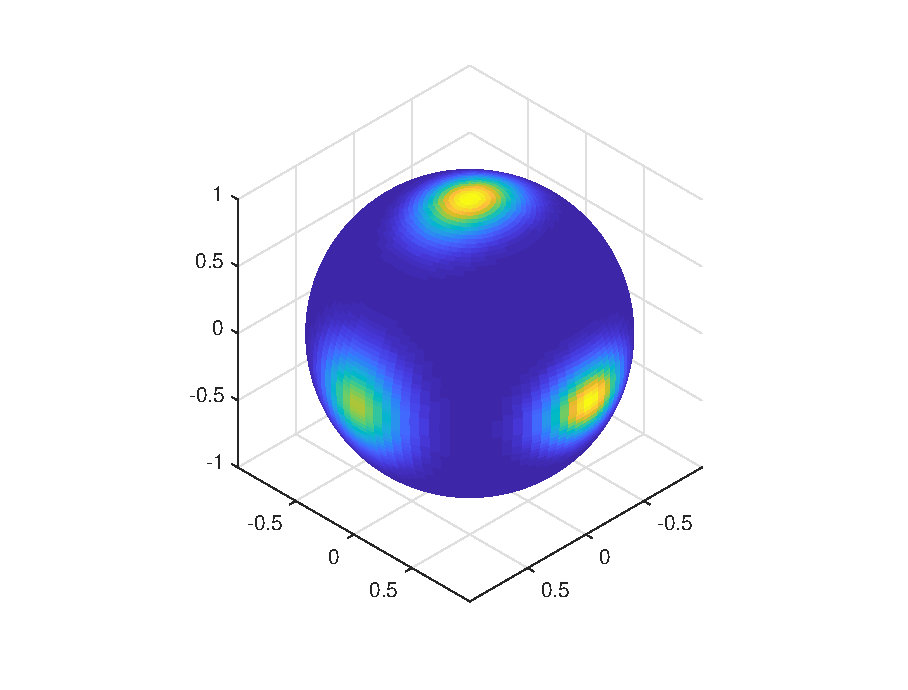
\includegraphics[height=2in]{x0}
		\caption{correlation $\bm{t}_x$, $x_1=0$}
	\end{subfigure}
	\begin{subfigure}{0.3\textwidth}
		\centering
		\includegraphics[height=2in]{y0}
		\caption{correlation $\bm{t}_y$, $x_1=0$}
	\end{subfigure}
	\begin{subfigure}{0.3\textwidth}
		\centering
		\includegraphics[height=2in]{z0}
		\caption{correlation $\bm{t}_z$, $x_1=0$}
	\end{subfigure}
	
	\begin{subfigure}{0.3\textwidth}
		\centering
		\includegraphics[height=2in]{x1}
		\caption{correlation $\bm{t}_x$, $x_1=1$}
	\end{subfigure}
	\begin{subfigure}{0.3\textwidth}
		\centering
		\includegraphics[height=2in]{y1}
		\caption{correlation $\bm{t}_y$, $x_1=1$}
	\end{subfigure}
	\begin{subfigure}{0.3\textwidth}
		\centering
		\includegraphics[height=2in]{z1}
		\caption{correlation $\bm{t}_z$, $x_1=1$}
	\end{subfigure}
	
	\begin{subfigure}{0.3\textwidth}
		\centering
		\includegraphics[height=2in]{x-1}
		\caption{correlation $\bm{t}_x$, $x_1=-1$}
	\end{subfigure}
	\begin{subfigure}{0.3\textwidth}
		\centering
		\includegraphics[height=2in]{y-1}
		\caption{correlation $\bm{t}_y$, $x_1=-1$}
	\end{subfigure}
	\begin{subfigure}{0.3\textwidth}
		\centering
		\includegraphics[height=2in]{z-1}
		\caption{correlation $\bm{t}_z$, $x_1=-1$}
	\end{subfigure}
	
	\caption{Matrix-Fisher Gaussian distribution on $\mathrm{SO}(3)\times\mathbb{R}$. \label{fig:SO3Correlation}}
\end{figure*}

\end{document}

